\documentclass[accentcolor=tud6b,11pt,paper=a4]{tudreport}

\usepackage[T1]{fontenc} 
\usepackage[utf8]{inputenc} 
\usepackage[ngerman]{babel}
\usepackage{listings}
\usepackage{pdfpages}

%======================================================
% KOM-modifications of the TUD-layout
%======================================================
% reduce font size of page footers and headers (fancyhdr)
\renewcommand{\footerfont}{\fontfamily{\sfdefault}\fontseries{m}\fontshape{n}\footnotesize\selectfont}
% remove space between items 
\usepackage{enumitem}
	\setenumerate{noitemsep}
	\setitemize{noitemsep}
	\setdescription{noitemsep}
%\setlist{nolistsep}

%======================================================
% Package loading for example contents (content.tex)
%======================================================
\usepackage{tabularx} % better tables
\setlength{\extrarowheight}{3pt} % increase table row height
\usepackage{booktabs}
\usepackage{caption}
\captionsetup{format=hang,font=small}
\usepackage[square,numbers]{natbib}
\usepackage{subfig}
\usepackage[stable,bottom]{footmisc}

%======================================================
% Setup for hyperref
%======================================================
\usepackage[pdftex,hyperfootnotes=true,pdfpagelabels]{hyperref}
\pdfcompresslevel=9
\pdfadjustspacing=1 
\hypersetup{
    pdftitle={XGVisualize, Ausarbeitung},%
    pdfauthor={Michael Bräunleinr, DKE, TU Darmstadt}
}

%============================================
% Setup of the title page (do not change)
%============================================
\title{Klassifikation der Schwierigkeitsgrade von Sudokus mit Methoden des maschinellen Lernens}
\subtitle{Investigation of Sudoku difficulty levels}
\subsubtitle{Bachelor-Thesis von Michael Bräunlein}
\institution{\raggedleft Fachbereich Informatik \\
	Knowledge Engineering Group
	Betreuer Prof. Dr. Johannes Fürnkranz
}
	
\begin{document}

\maketitle

% ===== abstract ==========================================
\begin{abstract}
Das Zahlenrätsel Sudoku ist weltweit bei Rätselliebhabern bekannt und beliebt. Seit seiner Veröffentlicheung 1986 begeistern sich immer mehr Menschen für mehr oder weniger schwierige Exemplare. Sudokus finden sich im Internet, in der Rätselecke der Tageszeitungen und sogar als ganze Bücher, um nur einige Erscheinungsorte zu nennen. \\
Die Regeln sind einfach zu lernen und doch kann man sich sehr lange mit Sudokus beschäftigen, da die schwersten Sudokus meißt nur von Profis gelöst werden können.\\
Der Spielspass ist sehr stark davon abhängig, dass die Schwierigkeit zum persönlichen Können passt. Ist das Sudoku zu leicht, stellt es keine Herausforderung dar. Ist es zu schwer, kommt schnell ein Gefühl der überforderung auf. \\
Die ausgewiesenen Schwierigkeitsstufen von Sudokus aus verschiedenen Quellen haben zwar of die gleeichen Namen wie zum Beispiel 
\textquotedblleft Mittel\textquotedblright
, unterscheiden sich aber dennoch häufig nach Meinung des Spielers.\\
Das Ziel dieser Bachelorarbeit ist, Merkmale aus Sudokus zu extrahieren, anhand derer die Sudokus von einem Klassifizierer möglichst zuverlässig in Schwierigkeitsstufen eingeteilt werden können.\\
\end{abstract}

% ===== lists =============================================
\tableofcontents

\chapter{Aufgabenstellung und Zielsetzung}
Diese Bachelorarbeit beschäftigt sich mit der Einteilung von Sudokus in verschiedene Schwierigkeitsstufen. Hierzu sollen Methoden des maschinellen Lernens verwendet werden. \\ Es soll eine Methode gefunden werden, mit der Merkmale aus Sudokus extrahiert werden können, die dann als Feature Vectoren in einer .arff Datei\footnote{\url{http://www.cs.waikato.ac.nz/ml/weka/arff.html}} gesammelt werden. Die Feature Vectoren werden anschließend mit Hilfe von Weka\footnote{\url{http://www.cs.waikato.ac.nz/ml/weka/}} klassifiziert.\\
Es werden verschiedene Klassifikatoren und unterschiedliche Parameter betrachtet. Ausserdem werden Optimierungen der Featurevektoren diskutiert.


%======================================================

\chapter{Einführung}
Die Vorfahren des heutigen Sudokus waren vermutlich die lateinischen Quadrate, mit denen sich vor allem der Mathematiker Leonhard Euler befasste. Hier ging es darum, in ein Quadrat mit n Zeilen und n Spalten Symbole so einzutragen, dass jedes Symbol in jeder Spalte und Zeile jeweils genau einmal vorkommt.

\begin{figure}[htbp]
\begin{center}
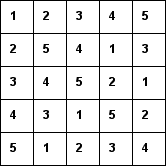
\includegraphics{./img/lat_quadrat.png}
\caption{Lateinisches Quadtrat}
\end{center}
\end{figure}

Daraus hat sich das heutige Sudoku entwickelt, das sich nicht nur bei Mathematikern großer Beliebtheit erfreut.

\section{Die Regeln}
Diese Arbeit beschäftigt sich nur mit der meist verbreiteten Art von Sudokus. Dabei spielt man auf einem 9x9 Felder großen Spielfeld, das wiederum in neun 3x3 Felder große Blöcke eingeteilt ist. Weiter handelt es sich nur dann um ein Sudoku, wenn genau eine Lösung vorhanden ist.
Ein Sudoku gilt dann als gelöst, wenn jede Zeile, jede Spalte und jeder Block die Ziffern 1 bis 9 genau einmal enthält.\\
\begin{figure}[h]
\begin{center}
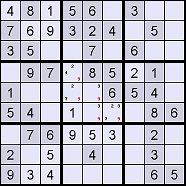
\includegraphics{./img/sudoku.jpg}
\caption{Sudoku}
\end{center}
\end{figure}


\section{Begriffserklärung}
Ein Sudoku besteht aus 81 \textit{Feldern} oder \textit{Zellen}. Diese bilden ein Quadrat der Größe 9x9, das \textit{Grid}. Aufgrund dieser Aufteilung hat ein Sudoku 9 \textit{Zeilen} und 9 \textit{Spalten}. Das Grid wird in 9 Unterquadrate geteilt, die jeweils 3x3 Felder groß sind. Diese werden \textit{Blöcke} genannt. Zeilen, Spalten und Blöcke werden unter dem Begriff \textit{Figur} zusammengfasst. Die Nummerierung der Blöcke erfolgt zeilenweise von links oben nach rechts unten.\\
\textit{Vorgaben} sind Zahlen, die schon von Anfang an gegeben sind.\\
In \textbf{Abbildung 2.2} sieht man im mittleren Block sogenannte \textit{Kandidaten}. Ein Kandidat ist eine Zahl, die in der Zelle noch möglich ist. Jede Zelle hat ihre eigene Liste mit Kandidaten.\\
In der Beschreibung der Lösungstechniken ist es notwendig bestimmte Felder zu betrachten. Hierzu wird eine Abkürzung verwendet, die Zeile und Spalte enthält und somit eine Zelle eindeutig indentifiziert. \textit{z2s3} meint zum Beispiel die Zelle in Zeile 2 und Spalte 3.\\
In der folgenden Abbildung sind die erläuterten Begriffe zum besseren Verständniss eingetragen.\\

\begin{figure}[h]
\begin{center}
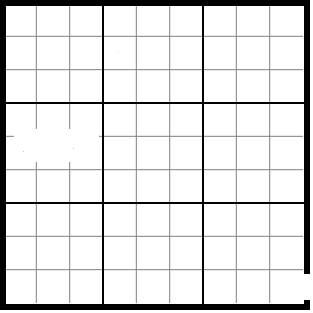
\includegraphics{./img/begriffe.png}
\caption{Begriffe}
\end{center}
\end{figure}
%======================================================

\chapter{Lösungsmethoden}
Alle in dieser Bachelorarbeit beschriebenen Techniken sind nicht im Rahmen dieser Arbeit entwickelt worden, sondern wurden aus verschiedenen Quellen zusammengetragen. Die Beschreibung der Lösungstechniken lehnt sich an die Beschreibung der Quellen an. Teile der Beispiele wurden aus den Quellen entnommen, dies ist entsprechend gekennzeichnet.\\
Grob kann man die Techniken zum Lösen von Sudokus in zwei Kategorien einteilen. Die erste Kategorie findet Zahlen heraus, die direkt in das Sudoku eingetragen werden können. Die Techniken der zweiten Kategorie entfernen Bedingungen in einzelnen Zellen des Sudokus.

\section{Kandidatenlisten}
Beim Lösen von Sudokus ist es üblich, in jedes Feld die Kandidaten einzutragen, die dort stehen können. Dabei wird vorerst nur die Sudoku Regel berücksichtigt, die besagt, dass in jeder Figure die Zahlen 1 bis 9 vorkommen müssen. Wenn in einer Zeile nun die Zahl 3 vorkommt, dann kann sie in der selben Zeile nicht nochmal vorkommen, daher kann sie aus allen Kandidatenlisten der Zellen in der selben Zeile gelöscht werden. Dasselbe gilt für Spalten und Blöcke. Immer wenn eine Ziffer in ein Feld eingetragen wird, dann muss der Spieler die Liste der Kandidaten aktualisieren.\\
Kandidatenlisten sind keine eigene Lösungstechnik, sind aber wesentlicher Bestandteil vieler Techniken.

\newpage
\section{Full House}
Wenn in einer Figur 8 Zahlen eingetragen sind, dann kann die Technik \textit{Full House} angewendet werden. Da in jeder Figur die Zahlen 1 bis 9 stehen müssen, kann die fehlende Zahl einfach per Ausschluss ermittelt werden.\\

\begin{figure}[h]
\begin{center}
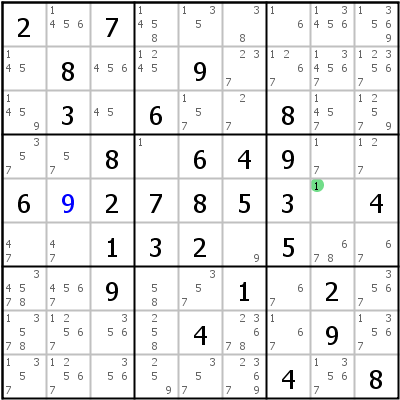
\includegraphics{./img/full_house.png}
\caption{Full House}
\end{center}
\end{figure}

In \textbf{Abbildung 3.1} fehlt in Zeile 5 nur noch eine Ziffer. Da die Zahlen 2 bis 9 bereits vorhanden sind, kann in das Feld z5s8 die Zahl 1 eingetragen werden.
\newpage
\section{Naked Single}
Bei der Technik \textit{Naked Single} werden Kandidatenlisten verwendet. Diese Technik kann angewendet werden, wenn in der Kandidatenliste einer Zelle nur noch ein Kandidat steht. Dieser Kandidat kann dann in die Zelle eingetragen werden. Das funktioniert aufgrund des Aufbaus der Kandidatenlisten. Diese enthalten zuerst alle Kandidaten und es werden immer dann Kandidaten entfernt, wenn dieser Kandidat nicht mehr als Ziffer in der Zelle stehen könnte wel er dort eine Regel verletzen würde. Wenn also nur noch ein Kandidat in der Kandidatenliste steht, dann bedeutet das, dass dieser Kandidat die einzige Ziffer zwischen 1 und 9 ist, die in der Zelle stehen kann ohne eine Regel zu verletzen.

\begin{figure}[h]
\begin{center}
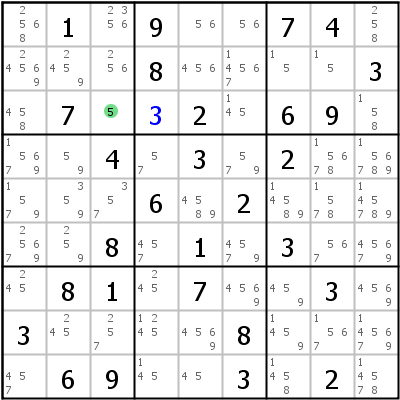
\includegraphics{./img/naked_single.png}
\caption{Naked Single}
\end{center}
\end{figure}

Im oben stehenden Beispiel \textbf{Abbildung 3.2} sieht man sofort, dass die Kandidatenliste in z3s3 nur noch einen Eintrag enthält. Dieser kann nun einfach eingetragen werden.
\newpage
\section{Hidden Single}
Auch die Technck \textit{Hidden Single} arbeitet wieder mit Kandidatenlisten. Wenn in einer Figur eine Kandidatenliste die einzige ist, in der eine bestimmte Zahl vorkommt, dann kann diese Zahl direkt in die Zelle eingetragen werden. Wenn in dieser Zelle die Zahl nicht stünde, dann gäbe es in der Figur keine Möglichkeit mehr, dass die Zahl auftaucht und damit wäre die Sudoku Regel verletzt, nach der jede Zahl genau einmal enthalten sein muss.

\begin{figure}[h]
\begin{center}
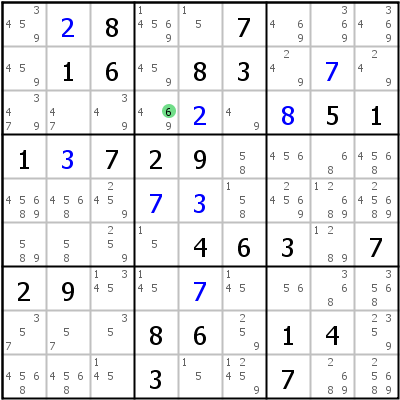
\includegraphics{./img/hidden_single.png}
\caption{Hidden Single}
\end{center}
\end{figure}

In \textbf{Abbildung 3.3} sieht man, dass die Zahl 6 in der Zeile 3 nur in z3s4 vorkommen kann. Daher kann man sie dort eintragen.

\newpage
\section{Pointing Pair / Triple}
Bei der Technik \textit{Pointing Pair / Triple} müssen zum ersten mal die Kandidatenlisten mehrerer Felder gleichzeitig betrachtet werden, was diese Technik etwas schwerer macht. Ausserdem ist diese Technik die erste, die Kandidaten aus Kandidatenlisten entfernt und nur bedingt zum Einsetzen von Zahlen in das Sudoku führt.\\
Es werden die Kandidatenlisten in Blöcken jeweils zeilen- und spaltenweise betrachtet. Die Technik \textit{Pointing Pair / Triple}
kann angewendet werden, wenn in einem Block eine Kandidat nur in Kandidatenlisten der selben Zeile oder Spalte vorkommt. Dann kann jedes weitere vorkommen der Zahl in einer Kandidatenliste der selben Zeile oder Spalte entfernt werden. Das gilt, da die Zahl genau einmal in dem Block vorkommen muss. Da alle möglichen Vorkommen der Zahl in der selben Zeile oder Spalte liegen ist klar, dass die Zahl in dieser Zeile oder Spalte vorkommt. Da sie aber kein zweites mal in der Zeile oder Spalte vorkommen darf muss sie aus den Kandidatenlisten entfernt werden, die nicht im selben Block liegen.

\begin{figure}[h]
\begin{center}
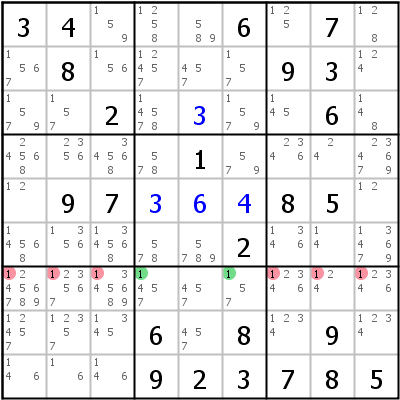
\includegraphics{./img/pointing_pair_triple.png}
\caption{Pointing Pair / Triple}
\end{center}
\end{figure}

In \textbf{Abbildung 3.4} betrachten wir Block 8. Hier ist das Vorkommen der Zahl 1 in den Kandidatenlisten auf Zeile 7 beschränkt. Wie oben beschrieben können nun alle weiteren vorkommen in der selben Zeile, die nicht in Block 8 liegen aus den Kandidatenlisten entfernt werden. Im vorliegenden Beispiel führt das allerdings nicht dazu, dass eine neue Zahl in das Sudoku eingetragen wird. Dennoch ist das Sudoku nun genauer bestimmt, da weniger Möglichkeiten übrig sind.

\newpage
\section{Box-Line Reduction}
\section{Naked Subset}
\section{Hidden Subset}
\section{Fish}
\subsection{X-Wing}
\subsection{Swordfish}
\subsection{Jellyfish}
\section{Single Digit Patterns}
\subsection{Skyscarper}
\subsection{2-String Kite}
\subsection{Turbot Fish}
\subsection{Empty Rectangle}
\section{Wings}
\subsection{XY-Wing}
\subsection{XYZ-Wing}
\subsection{W-Wing}
\section{Sue de Coq}
\section{Coloring}
\section{Almost Locked Set}
\subsection{ALS XZ}
\subsection{ALS XY Wing}
\subsection{ALS Chain}

%======================================================

\chapter{Merkmalsextrahierung}
\section{Allgemeines Vorgehen}
\section{Entkopplung von konkreten Zahlen}
%======================================================

\end{document}